
%\documentclass[calculator,fluidstables,datasheet,solutions,resit]{exam}
%\documentclass[calculator,fluidstables,datasheet,resit]{exam}
\documentclass[calculator,fluidstables,datasheet,sample]{exam}

% The full list of class options are
% calculator : Allows approved calculator use.
% datasheet : Adds a note that data sheet are attached to the exam.
% handbook : Allows the use of the engineering handbook.
% resit : Adds the resit markings to the paper.
% sample : Adds conspicuous SAMPLE markings to the paper
% solutions : Uses the contents of \solution commands (and \solmarks) to generate a solution file

\usepackage{pdfpages} 
\usepackage{lscape,comment}



\coursecode{EG3029}%%

\examtime{00.00--00.00}%
\examdate{00}{01}{2015}%
\examformat{Candidates must attempt \textit{all} questions.}

\newcommand{\frc}{\displaystyle\frac}
\newcommand{\br}[1]{\!\left( #1 \right)}
\newcommand{\abs}[1]{\left| #1 \right|}
\newcommand{\fracd}[2]{\frac{\mathrm{d} #1}{\mathrm{d} #2}}
\newcommand{\fracp}[2]{\frac{\partial #1}{\partial #2}}
\renewcommand{\d}[1]{\mathrm{d} #1 } 
\newcommand{\Ma}{\mathrm{M\!a}} 


\begin{document}
%%%
%%% Question 01 
%%%
\begin{question}

Steam is produced in a boiler at 60 bar and 335$^{\circ}$C . The fluid is driven into a turbine where an isentropic expansion take place with efficiency of 75$\%$. Before re-vaporisation in the boiler, the fluid is condensed in a heat exchanger, where the extracted energy is used to heat up a stream of NH$_{3}$ at 15$^{\circ}$C. The mass flow rate of water and NH$_{3}$ are 20 and 220 kg.s$^{-1}$, respectively. Assume that the pump has 100$\%$ of efficiency.
\begin{center}
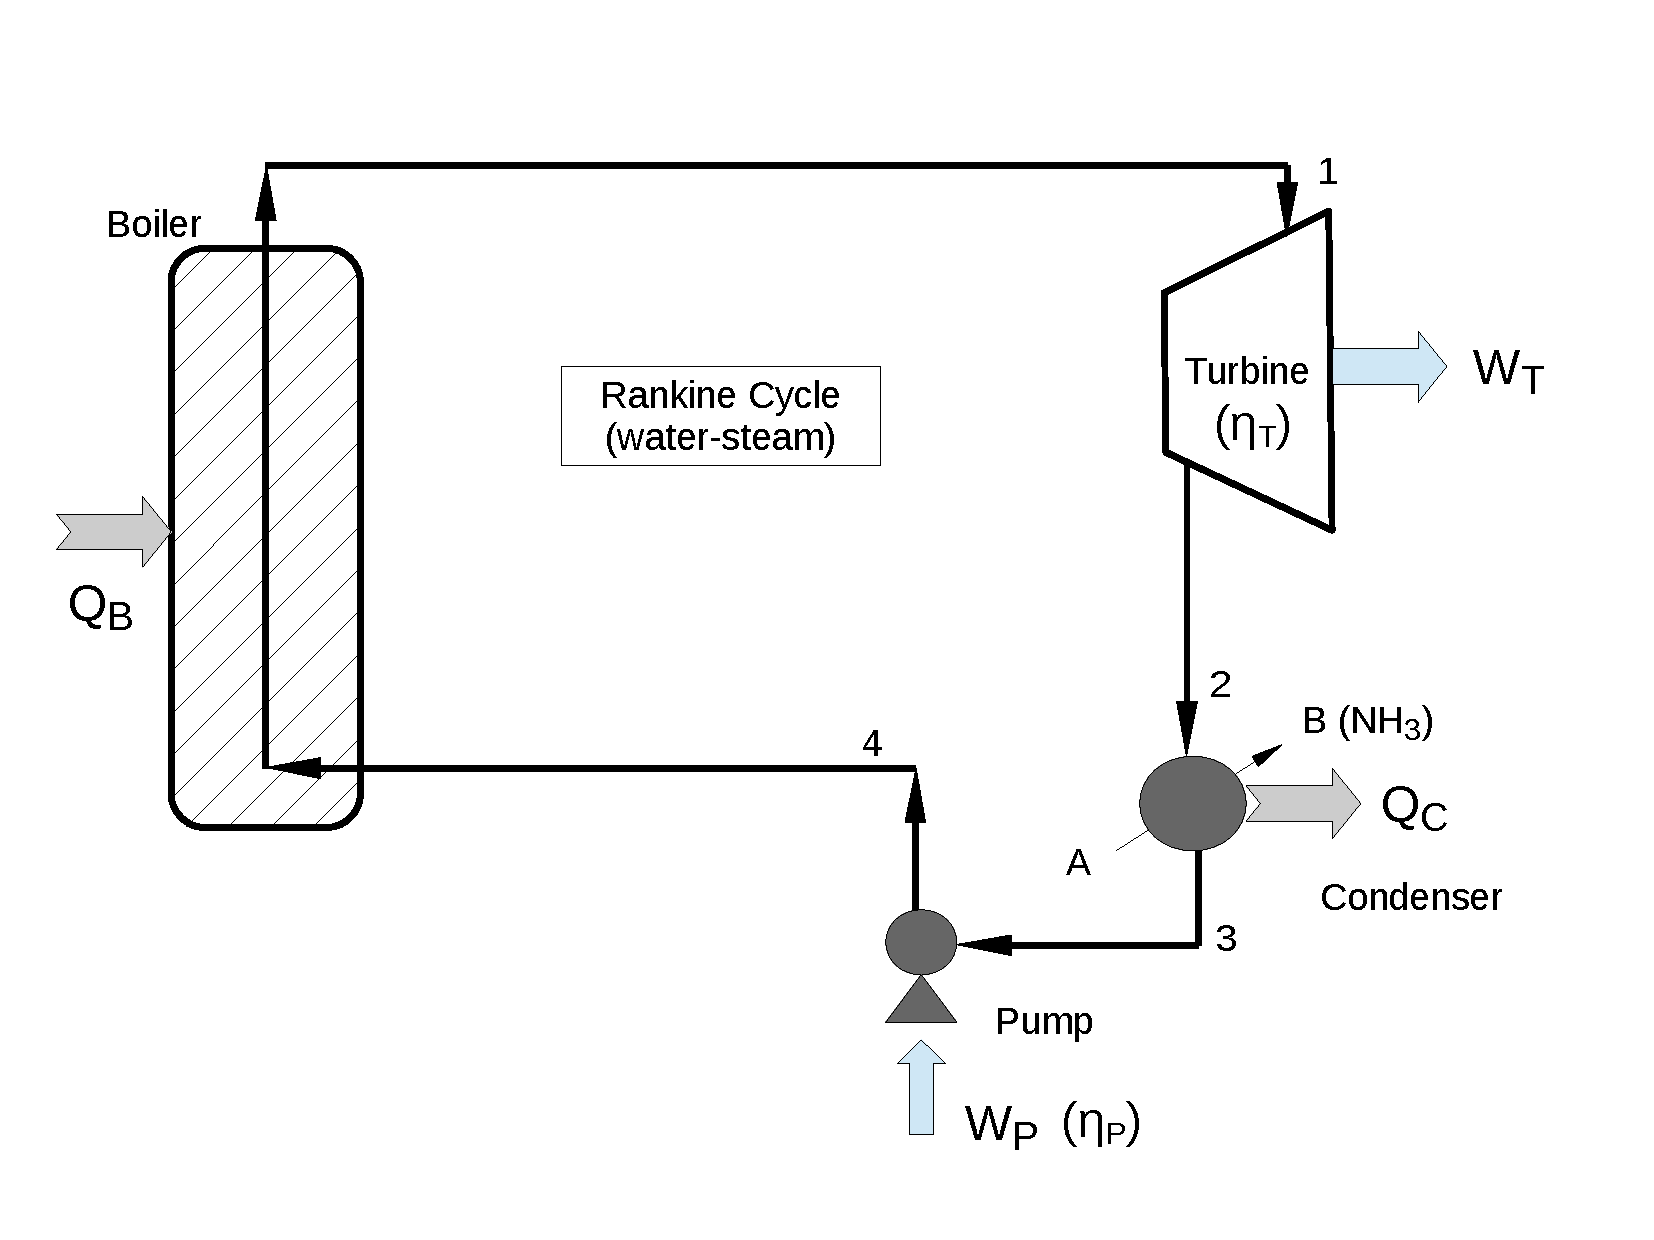
\includegraphics[width=12.cm,height=8.cm,clip]{./Pics/RankineCycle2_Sample}
%\caption{ Reheat and regenerative Rankine cycle with 2 turbines.}
\label{exam_mod02_rankinecycle}
\end{center}
\begin{enumerate}
\item Calculate (a-k) in the table below.~\marks{11}
\item Calculate the power produced in the turbine $\left(\dot{W}_{T}\right)$ and the heat extracted in the condenser $\left(\dot{Q}_{C}\right)$.~\marks{2}
\item Sketch the $TS$ diagram indicating all stages of the thermal cycle.~\marks{4}
\item Calculate the efficiency of the cycle $\left(\eta_{\text{cycle}}=\frc{\dot{W}_{\text{net}}}{\dot{Q}_{B}}\right)$~\marks{3}
\end{enumerate}
\begin{center}
\begin{tabular} {||c | c c c c c c || }
\hline\hline
{\bf Stage} & {\bf P}    & {\bf T}        & {\bf State}    & {\bf H}             & {\bf S}                 &  {\bf Quality of the} \\
            & {\bf (bar)}& {\bf ($^{o}$C)} &               & {\bf (kJ.kg$^{-1}$)} & {\bf (kJ.(kg.K)$^{-1}$)} &  {\bf vapour $\left(x_{i}\right)$} \\
\hline\hline
 {\bf 1 }   & 60         & 335            &   {\bf (a)}    & {\bf (b)}           & {\bf (c)}               &   --          \\
 {\bf 2 }   & 4.50       &  --            &   wet vapour   & {\bf (d)}           & {\bf (e)}               &   {\bf (f)}    \\
 {\bf 3 }   & --         &                &   sat. liquid  & {\bf (g)}           & {\bf (h)}               &   --            \\
 {\bf 4 }   & --         &                &   {\bf (i)}    & {\bf (j)}           & --                      &   --            \\
 {\bf A }   & --         & 15             &   --           & --                  & --                      &   --     \\
 {\bf B }   & --         & {\bf (k)}      &   --           & --                  & --                      &   --         \\
 \hline\hline
\end{tabular}
\end{center}
%
\end{question}
\clearpage

%%%
%%% Question 02
%%%
\begin{question}
\begin{enumerate}
\item\label{Tut01:FirstLawIdealGas2} Given air (assuming ideal gas behaviour) expanding reversibly and adiabatically from $T_{1}=450 K$ and $V_{1}=3.0\times 10^{-3}m^{3}$ to the final volume, $V_{2}=5.0\times 10^{-3}m^{3}$. %$T$ and $V$ relationship for constant heat capacities is represented by $\displaystyle\frc{T_{2}}{T_{1}} = \left(\frc{V_{1}}{V_{2}}\right)^{\gamma-1}$.
\begin{enumerate}
\item Derive a relationship between $T$ and $P$; Assuming that $C_{p}= 5.0 cal.\left(mol.K\right)^{-1}$ and $C_{v}=3.0 cal.\left(mol.K\right)^{-1}$;~\marks{5}
\item Calculate $T_{2}$;~\marks{3}
\item Calculate the work done during the process and;~\marks{2}
\item Determine the enthalpy change.~\marks{2}
\end{enumerate}

%%%
%%% Johannes T3Q4
%%%
\item\label{Tut02:Demonstration}Assuming $S = S\left(P,V\right)$ and taking into consideration that,
\begin{displaymath}
\left(\frc{\partial S}{\partial T}\right)_{V} = \frc{C_{V}}{T}\;\;\;\text{ and }\;\;\; \left(\frc{\partial S}{\partial T}\right)_{P} = \frc{C_{P}}{T}
\end{displaymath}
Prove that 
\begin{displaymath}
\d S = \frc{C_{V}}{T}\left(\frc{\partial T}{\partial P}\right)_{V}\d P + \frc{C_{P}}{T}\left(\frc{\partial T}{\partial V}\right)_{P}\d V
\end{displaymath}~\marks{8}

\end{enumerate}
\end{question}
\clearpage

%%%
%%% Question 03
%%%
\begin{question}
\begin{enumerate}
\item\label{prove} For $\beta = \frc{1}{V}\left(\frc{\partial V}{\partial T}\right)_{P}$ (volume expansivity) and $\kappa = -\frc{1}{V}\left(\frc{\partial V}{\partial P}\right)_{T}$ (isothermal compressibility), demonstrate that $\left(\frc{\partial\beta}{\partial P}\right)_{T} = -\left(\frc{\partial\kappa}{\partial T}\right)_{P}$. Hint: consider $V=V\left(T,P\right)$.~\marks{8}
%%%
%%% Johannes T4Q2
%%%
\item\label{Tut03:EOS1} Calculate $V$ and $Z$ for sulphur hexafluoride at 75$^{\circ}$C and 15 bar using the Peng-Robinson equation of state. Given: P$_{c}$ = 37.6 bar, T$_{c}$ = 318.7 K, V$_{c}$ = 198 cm$^{3}$.gmol$^{-1}$, $\omega$ = 0.286.~\marks{12}
\end{enumerate}
\end{question}

\clearpage
%%%
%%% Question 04
%%%
\begin{question}
\begin{enumerate}

%%%
%%% Johannes Problem 2 (Tutorial 5)
%%%
\item\label{Tut05P2} A process stream contains light species 1 and heavy species 2. A relatively pure liquid stream containing mostly 2 is obtained through a single-stage liquid/vapour separator. Specifications on the equilibrium composition are: $x_{1}$ = 0.002 and $y_{1}$ = 0.950. Assuming that the modified Raoult's law applies, 
\begin{displaymath}
  y_{i} P = x_{i}\gamma_{i}P_{i}^{\text{sat}}
\end{displaymath} 
Determine $T$ and $P$ for the separator. Given the activity coefficients for the liquid phase,
\begin{displaymath}
\ln\gamma_{1} = 0.93x_{2}^{2} \;\;\;\;\;\text{ and }\;\;\;\;\;\ln\gamma_{2}=0.93x_{1}^{2}
\end{displaymath}
\begin{displaymath}
\ln P^{\text{sat}} = A - \frc{B}{T}\;\;\;\text{with [P] = bar and [T] = K}
\end{displaymath} 
$A_{1}$= 10.08, $B_{1}$ = 2572.0, $A_{2}$ = 11.63 and $B_{2}=6254.0$.~\marks{10}

\item\label{SMVN} For the acetone (Ket) / methanol (MetOH) system, a vapour mixture of $z_{\text{Ket}}$ = 0.25 and $z_{\text{MetOH}}$ = 0.75 is cooled to temperature $T$ in the two-phase region and flows into a separation chamber at a pressure of 1 bar. If the composition of the liquid product is $x_{\text{Ket}}$ = 0.175, calculate $T$  and $y_{\text{Ket}}$. For liquid mixture, assume that
\begin{displaymath}
\ln\gamma_{1} = 0.64x_{2}^{2} \;\;\;\;\;\text{ and }\;\;\;\;\;\ln\gamma_{2}=0.64x_{1}^{2}
\end{displaymath}
For the Antoine equation, 
\begin{displaymath}
\ln P_{i}^{\text{sat}} = A_{i} - \frc{B_{i}}{T + C} \;\;\left(\text{ [P] = kPa and [T] = }^{\circ}\text{C}\right)
\end{displaymath}
$A_{\text{Ket}}$ = 14.3145, $B_{\text{Ket}}$ = 2756.22, $C_{\text{Ket}}$ = 228.060, $A_{\text{MetOH}}$ = 16.5785, $B_{\text{MetOH}}$ = 3638.27, $C_{\text{MetOH}}$ = 239.50.~\marks{10}

\end{enumerate}
\end{question}

\clearpage
\begin{question}
\begin{enumerate}
\item The volume change of mixing $\left(\text{cm}^{3}.\text{gmol}^{-1}\right)$ for the system ethanol (1) / methyl-butyl ether (2) at 25$^{\circ}$C is given by the equation:
\begin{displaymath}
\Delta V = x_{1}x_{2}\left[-1.026+0.220\left(x_{1}-x_{2}\right)\right]
\end{displaymath}
Given that V$_{1}$ = 58.63 cm$^{3}$.gmol$^{-1}$ and V$_{2}$ = 118.46 cm$^{3}$.gmol$^{-1}$, what volume of mixture is formed when 750 cm$^{3}$ of pure species 1 is mixed with 1500 cm$^{3}$ of species 2 at 25$^{\circ}$C? What would be the volume if an ideal solution were formed?~\marks{8}

\item In a reactor, 2 mol carbon dioxide, 5 mol hydrogen and 1 mol carbon monoxide are mixed and start to undergo the reactions:
\begin{eqnarray}
CO_{2} + 3 H_{2} &\rightarrow& CH_{3}OH +H_{2}O\nonumber \\
CO_{2} + H_{2}  &\rightarrow& CO + H_{2}O\nonumber
\end{eqnarray}
Develop expressions for the mole fractions of the reacting species as functions of the reaction coordinates for the two reactions.~\marks{12}

\end{enumerate}
\end{question}

\clearpage
\begin{itemize}
%%%
\item Generic cubic equation of state:
\begin{eqnarray}
&& Z= 1 + \beta - q\beta \frc{Z - \beta} {\left(Z+\varepsilon\beta\right)\left(Z+\sigma\beta\right)}  \;\;\text{(vapour and vapour-like roots)}\nonumber\\
&& Z= 1 + \beta + \left(Z + \epsilon\beta\right)\left(Z+\sigma\beta\right)\left(\frc{1+\beta-Z}{q\beta}\right)  \;\;\text{(liquid and liquid-like roots)}\nonumber\\
&& \text{with }\; \beta=\Omega\frc{P_{r}}{T_{r}} \;\;\text{ and } \;\; q=\frc{\Psi\alpha\left(T_{r}\right)}{\Omega T_{r}}  \nonumber \\
&&\alpha_{\text{SRK}} = \left[ 1 + \left( 0.480 + 1.574 \omega - 0.176\omega^{2}\right)\left(1-\sqrt{T_{r}}\right)\right]^{2}  \nonumber \\
&&\alpha_{\text{PR}} = \left[ 1 + \left( 0.37464 + 1.54226 \omega - 0.26992\omega^{2}\right)\left(1-\sqrt{T_{r}}\right)\right]^{2} \nonumber
\end{eqnarray} 
    \begin{center}
       \begin{tabular}{| l | c c c c c| }
       \hline
          {\bf EOS}  & {\bf $\alpha$} & {\bf $\sigma$}  & {\bf $\varepsilon$} & {\bf $\Omega$} & {\bf $\Psi$ } \\
       \hline
            vdW      & 1              & 0               & 0                  & 1/8            & 27/64          \\
            RK       & T$_{r}^{-1/2}$  & 1                & 0                  & 0.08664       & 0.42748        \\
           SRK       &$\alpha_{\text{SRK}}$& 1            & 0                   & 0.08664       & 0.42748        \\
            PR       &$\alpha_{\text{PR}}$& 1+$\sqrt{2}$   & 1-$\sqrt{2}$        & 0.07780        & 0.45724  \\
       \hline
       \end{tabular}
    \end{center}

%%%
\item Newton-Raphson (root-finder) method: $X_{i} = X_{i-1} - \frc{\mathcal{F}\left(X_{i-1}\right)}{d\mathcal{F}/dX\left(X_{i-1}\right)}$

%%%
\item Fundamental thermodynamic equations:\\
\begin{tabular}{c c c c}
$dU = dQ + dW$;  & $dH = dU + d(PV)$; & $dA = dU -d(TS)$; & $dG=dH-d(TS)$ \\
$dU = TdS - PdV$;& $dH = TdS + VdP$;  & $dA = -SdT - PdV$;& $dG = -SdT + VdP$ \\ 
\end{tabular}\\
\begin{tabular} {c c}
$dH = C_{p}dT + \left[ V - T\left(\frc{\partial V}{\partial T}\right)_{P}\right]dP$; &  $dS=C_{p}\frc{dT}{T} - \left(\frc{\partial V}{\partial T}\right)_{P}dP$ \\
$dU = C_{v}dT + \left[T\left(\frc{\partial P}{\partial T}\right)_{V} - P\right]dV$;  & $dS = C_{v}\frc{dT}{T} - \left(\frc{\partial P}{\partial T}\right)_{V}dV$
\end{tabular}

%%% 
\item Polytropic Relations:\\
\begin{displaymath} 
\frc{T_{2}}{T_{1}} =\left(\frc{P_{2}}{P_{1}}\right)^{\frac{\gamma-1}{\gamma}} = \left(\frc{V_{1}}{V_{2}}\right)^{\gamma-1}\;\; ; 
TV^{\gamma-1} =\text{ const};\; TP^{\frac{1-\gamma}{\gamma}}=\text{ const};\; PV^{\gamma}=\text{ const} 
\end{displaymath}

%%%
\item Raoult's Law:\\
\begin{displaymath}
y_{i}P = x_{i}P_{i}^{\text{sat}}\;\;\;\text{ and } \;\;\; y_{i}P = x_{i}\gamma_{i}P_{i}^{\text{sat}}\;\;\;\text{ with } i=1,2,\cdots N
\end{displaymath}

%%%
\item Henry's Law:\\
\begin{displaymath}
x_{i}\mathcal{H}_{i} = y_{i}P\;\;\;\text{ with } i=1,2,\cdots N
\end{displaymath}

%%%
\item Antoine Equation:\\
\begin{displaymath}
\log_{10} P^{\star} = A-\frc{B}{T+C}\;\;\;\text{ with P}^{\star}\text{ in mm-Hg and T in }^{\circ}\text{C}
\end{displaymath}

%%%
\item Solutions:\\
\begin{displaymath}
M^{\text{E}} = M - \sum\limits_{i=1}^{N} x_{i}M_{i}; \; \overline{M}_{1}=M+x_{2}\frc{d M}{dx_{1}};\; \overline{M}_{2} = M - x_{1}\frc{d M}{dx_{1}}
\end{displaymath}

\end{itemize}

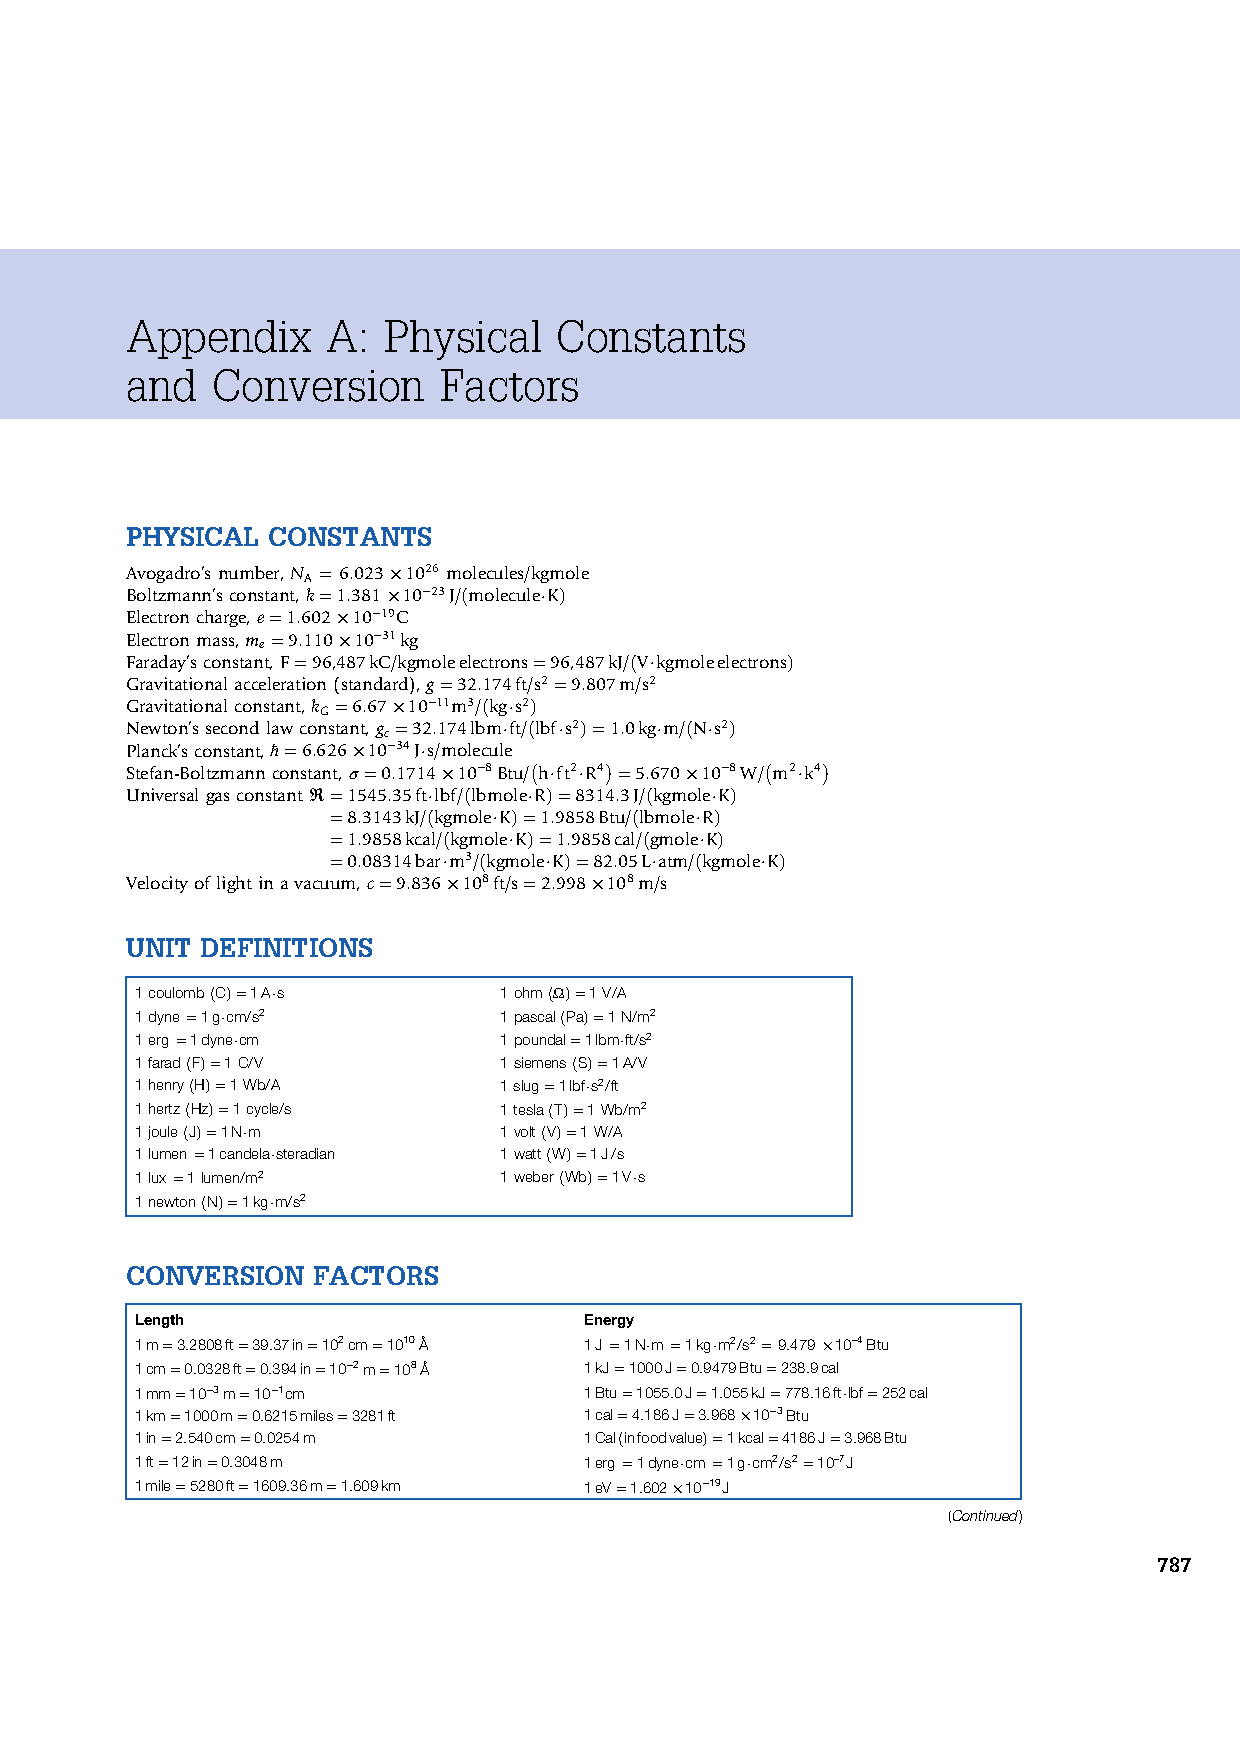
\includepdf[pages={1-10}]{./Pics/WaterSteam__UnitConv}

\clearpage
\end{document}
